% Copyright (C) 2005-2015 Airbus - EDF - IMACS - Phimeca
% Permission is granted to copy, distribute and/or modify this document
% under the terms of the GNU Free Documentation License, Version 1.2
% or any later version published by the Free Software Foundation;
% with no Invariant Sections, no Front-Cover Texts, and no Back-Cover
% Texts.  A copy of the license is included in the section entitled "GNU
% Free Documentation License".
\renewcommand{\filename}{docUC_StocProc_NormalProcess_Creation.tex}
\renewcommand{\filetitle}{UC : Creation of a normal process}

% \HeaderNNIILevel
% \HeaderIILevel
\HeaderIIILevel

\label{StationaryNormalProcessCreation}

\index{Stochastic Process!Normal Process}

This Use Case details how to create a  normal process $X: \Omega \times \cD \rightarrow \Rset^d$ either from its temporal covariance function or/and its spectral density function $S$ (when it exists). \\

A normal process defined by its temporal covariance function may have a trend: in that case, the normla process is the sum of the trend fucntion and a zero-mean normal process.\\

A zero-mean normal process is completely defined either by :
\begin{itemize}
\item its (temporal) covariance function   $C :   \cD\times \cD  \rightarrow  \mathcal{M}_{d \times d}(\Rset)$, which writes, in the stationary case: $C^{stat}:  \cD \rightarrow  \mathcal{M}_{d \times d}(\Rset)$.  In that case, the normal process is used through its temporal view only, thanks to the object {\itshape TemporalNormalProcess},
\item or its bilateral spectral density function (when it exists), in the stationary case,  $S : \Rset \rightarrow \mathcal{H}^+(d)$. In that case, the normal process is used through its spectral view only, thanks to the object {\itshape SpectralNormalProcess}. OpenTURNS restricts that possibility to processes for which the domain is of dimension 1: $\cD \in \Rset$ ($n=1$).
\end{itemize}

When the zero-mean process is stationary, in order to manipulate the same normal process through both the temporal and spectral views, it is necessary to create a second order model that insures the coherence between the covariance function $C^{stat}$  and the spectral density function $S$ through the relation (\ref{specdensFunc}). \\
In that purpose, the object {\itshape SecondOrderModel} is built (see the use case \ref{SecondOrderModel}) and then used to create a {\itshape TemporalNormalProcess} and the associated {\itshape SpectralNormalProcess} .\\
The choice between a {\itshape TemporalNormalProcess} and a {\itshape SpectralNormalProcess}  based on the same second order model is motivated by performance considerations of the specific algorithms either in terms of memory requirements and CPU requirements. For example, the performance of the algorithms related to the spectral density function (FFT) varies greatly if the number of frequencies is a power of 2 or not.\\

In the case of a {\itshape TemporalNormalProcess}, we can ask for the trend function of the process thanks to the method \emph{getTrend} or the covariance model and evaluate the covariance function  thanks to the method \emph{computeCovariance} or discretize  it on a specific mesh thanks to the method \emph{discretizeCovariance}, which creates the matrix defined in (\ref{covMatrix}).\\
In the case of a {\itshape SpectralNormalProcess}, we can ask for the spectral model and evaluate the bilateral spectral density function $S$ defined in (\ref{specdensFunc}) thanks to the method \emph{computeSpectralDensity}.\\

We note $N$ the number of vertices of the mesh $\cM$ on wich $\cD$ is discretized.\\
The first call to the method \emph{getRealization} implies different actions according to the type of the   normal process :
\begin{itemize}
\item in case of a {\itshape TemporalNormalProcess}, OpenTURNS builds the covariance matrix $\mat{C}_{1,\dots,N} \in \mathcal{M}_{Nd,Nd}(\Rset     )$ defined in (\ref{covMatrix}), using the  method \emph{discretizeCovariance}. Then $\mat{C}_{1,\dots,N}$ is factorized using the \emph{Cholesky} algorithm:  $\mat{C}_{1,\dots,N} = \mat{G} \, \mat{G}^{t}$.
\item in case of a {\itshape SpectralNormalProcess}, OpenTURNS builds the $n$ bilateral spectral density matrices $(\mat{S}(f_i))_{1 \leq i \leq,N}$ defined in (\ref{specdensFunc}) where $(f_i)_{1 \leq i \leq,N}$ are the frequencies associated to the time grid. Then each matrix $mat{S}(f_i)$ is factorized using the \emph{Cholesky} algorithm:  $\mat{S}(f_i) = \mat{H}_i \, \overline{\mat{H}}_i^{t}$.
\end{itemize}
These matrices $\mat{G}$ and $\mat{H}_i$ are used to get some realizations of the process from realizations of a standard normal process (with zero mean and unit covariance matrix). \\

In order to get the Cholesky factor of $\mat{C}_{1,\dots,N}$ or $(\mat{S}(f_i))_{1 \leq i \leq N}$, we might need to scale the matrices, due to some numerical precisions.
This scale consists in replacing the matrix $\mat{C}_{1,\dots,N}$ (resp. $\mat{S}(f_i)$) by $\mat{C}_{1,\dots,N} + \epsilon * \mat{I}$ (resp. $\mat{S}(f_i) + \epsilon * \mat{I}$) with  $\mat{I}$ the identity matrix and $\epsilon$ a negligible scalar variable. \\
In this case, the User gets a warning message to inform him about the used $\epsilon$ value to get the Cholesky factor.\\

\requirements{

  \begin{description}
  \item[$\bullet$] a mesh : {\itshape myMesh}
  \item[type:]  Mesh
  \end{description}

  \begin{description}
  \item[$\bullet$] a time grid : {\itshape myTimeGrid}
  \item[type:]  RegularGrid
  \end{description}

  \begin{description}
  \item[$\bullet$] a trend function : {\itshape myTrend}
  \item[type:] TrendTransform
  \end{description}

  \begin{description}
  \item[$\bullet$] covariance models : {\itshape myCovarianceModel}
  \item[type:] StationaryCovarianceModel
  \end{description}

  \begin{description}
  \item[$\bullet$] a spectral model : {\itshape mySpectralModel}
  \item[type:] SpectralModel
  \end{description}

  \begin{description}
  \item[$\bullet$] a second order model : {\itshape mySecondOrderModel }
  \item[type:] SecondOrderModel
  \end{description}

}
{

  \begin{description}
  \item[$\bullet$] normal processes : {\itshape myTempNormProc1, myTempNormProc2}
  \item[type:]  TemporalNormalProcess
  \end{description}

  \begin{description}
  \item[$\bullet$] the normal process : {\itshape mySpectNormProc1, mySpectNormProc2}
  \item[type:]  SpectralNormalProcess
  \end{description}
}

\textspace\\
Python script for this UseCase :\\

\inputscript{script_docUC_StocProc_NormalProcess_Creation}



The example illustrated below is a bivariate normal process with the Exponential model for the covariance one, parameterized by  $\vect{\lambda}=(1,1)$, $\vect{a}=(1,1)$ and $\mat{R}$ the identity matrix. We built a \textit{TemporalNormalProcess} and a \textit{SpectralNormalProcess} using the same \textit{SecondOrderModel} and the same \textit{RegularGrid}. Figures (\ref{temporalNormalProcess_Realization}) to (\ref{spectralNormalProcess_Realizations}) respectively draw the graphs of:
\begin{itemize}
\item  one realization of the temporal process (both marginals are illustrated),
\item   a sample of 5 realizations of the process (the first marginal is presented here) based on the covariance of the second order model,
\item  one realization of the spectral process (both marginals are illustrated),
\item  a sample of 5 realizations of the process (the first marginal is presented here) based on the spectral density of the second order model.
\end{itemize}

\begin{figure}[H]
  \begin{minipage}{9cm}
    \begin{center}
      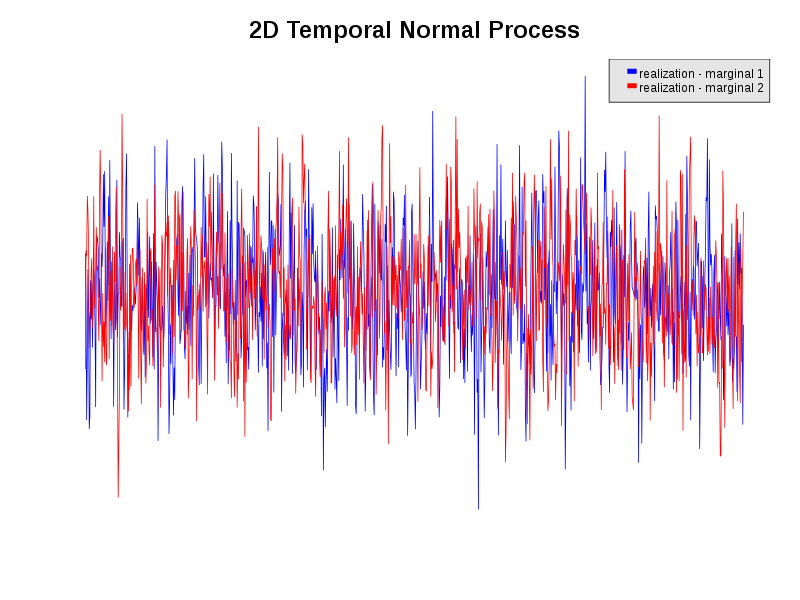
\includegraphics[width=7cm]{Figures/temporalNormal2D_realization.png}
      \caption{Realization of TemporalNormalProcess}
      \label{temporalNormalProcess_Realization}
    \end{center}
  \end{minipage}
  \hfill
  \begin{minipage}{9cm}
    \begin{center}
      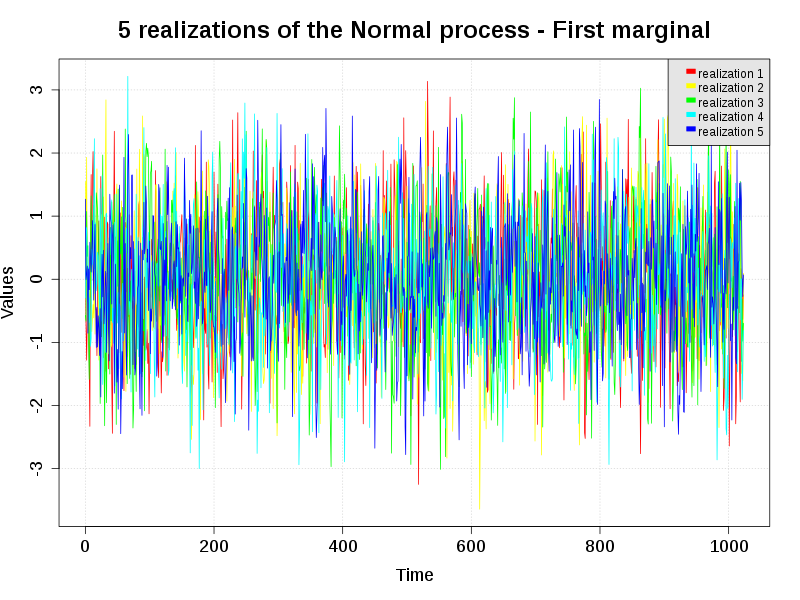
\includegraphics[width=7cm]{Figures/temporalNormal2D_realizations.png}
      \caption{$5$ realizations of the TemporalNormalProcess}
      \label{temporalNormalProcess_Realizations}
    \end{center}
  \end{minipage}
\end{figure}



\begin{figure}[H]
  \begin{minipage}{9cm}
    \begin{center}
      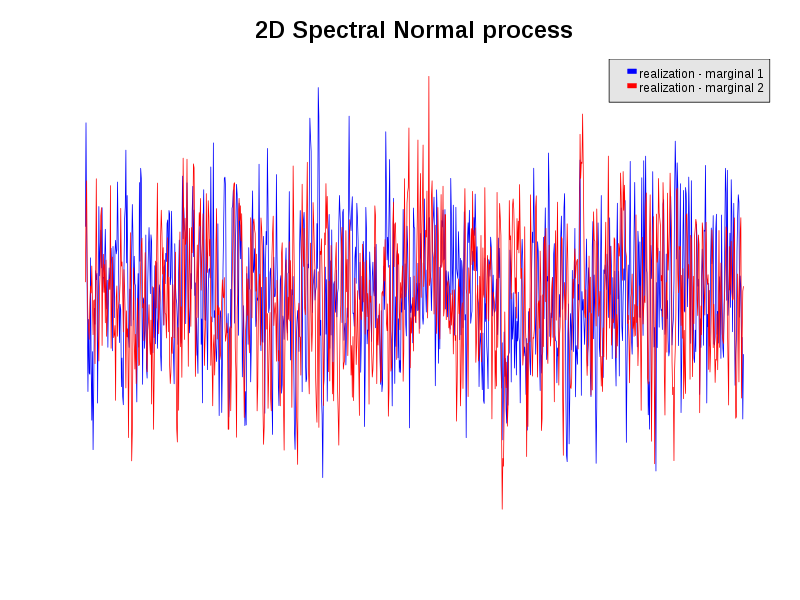
\includegraphics[width=7cm]{Figures/spectralNormal2D_realization.png}
      \caption{Realization of SpectralNormalProcess}
      \label{spectralNormalProcess_Realization}
    \end{center}
  \end{minipage}
  \hfill
  \begin{minipage}{9cm}
    \begin{center}
      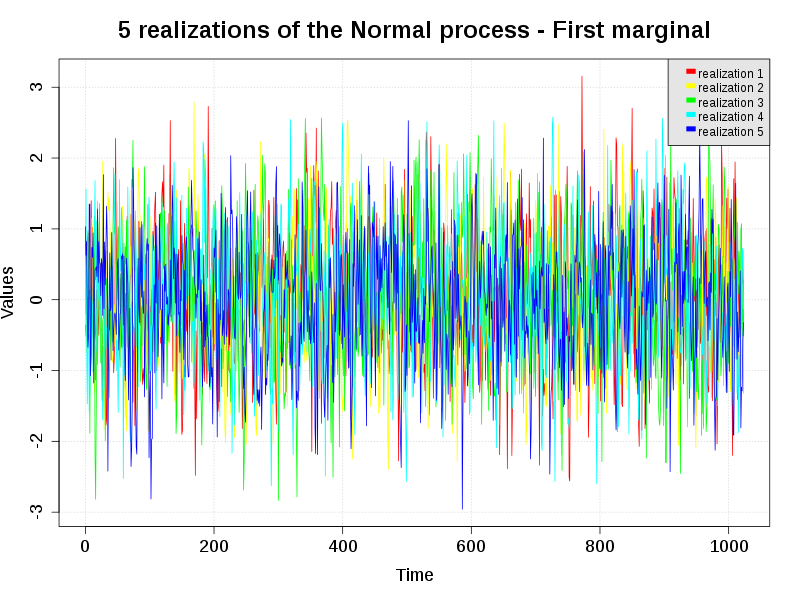
\includegraphics[width=7cm]{Figures/spectralNormal2D_realizations.png}
      \caption{$5$ realizations of the SpectralNormalProcess}
      \label{spectralNormalProcess_Realizations}
    \end{center}
  \end{minipage}
\end{figure}
